\documentclass{article}
\usepackage{graphicx}
\usepackage{amsmath}
\usepackage{amssymb}
\usepackage{physics}
\usepackage{hyperref}
\usepackage{float}
\usepackage[font=small]{caption}

\begin{document}

\section*{Problem 2: Fully Restrained Beam under Uniform Load}

\subsection*{Governing Equation}
The beam equation is identical to Problem 1:
\[
\frac{d^4 w}{dx^4} = -\frac{q}{EI}
\]
with identical parameters \( E \), \( I \), \( q \), and \( L \).

\subsection*{Boundary Conditions}
\begin{itemize}
    \item \textbf{Both ends} (\( x = 0 \) and \( x = L \)):
        \[
        w(0) = w(L) = 0, \quad \frac{dw}{dx}\Big|_{x=0} = \frac{dw}{dx}\Big|_{x=L} = 0
        \]
\end{itemize}

\subsection*{Analytical Solution}
\[
w_{\text{exact}}(x) = -\frac{q}{24EI} \left( x^4 - 2Lx^3 + L^2x^2 \right)
\]

\subsection*{PINN Implementation}
\begin{itemize}
    \item \textbf{Architecture}: FNN with 4 layers (1-50-50-50-1)
    \item \textbf{Activation}: Swish
    \item \textbf{Optimizer}: Adam (\( \text{lr} = 5 \times 10^{-5} \)) + L-BFGS
    \item \textbf{Loss}: PDE residual + 4 boundary conditions
    \item \textbf{Training}: 15,000 Adam + L-BFGS iterations
\end{itemize}

\begin{figure}[H]
    \centering
    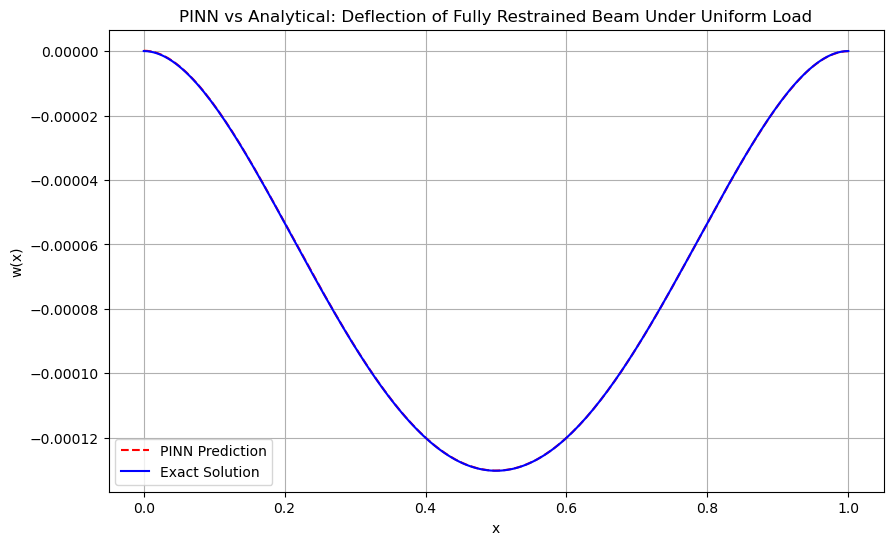
\includegraphics[width=0.8\textwidth]{geom2.png}
    \caption{PINN prediction vs analytical solution for fully restrained beam deflection}
    \label{fig:restrained}
\end{figure}

\end{document}